% Note: The content of this file was taken and adapted from Darwin Roduit's master thesis (June 2024).
% The algorithm was written based on documents of Yves Revaz. 
% The latex file was simplified to be part of SWIFT. 

\documentclass[a4paper]{ar-1col-S2O}

% Math packages
\usepackage{amsmath}
\usepackage{amssymb}
\usepackage{amsfonts}

% Physics package
\usepackage{physics}

% Algorithm packages
\usepackage{algorithm}
\usepackage{algpseudocodex} 

\begin{document}  %------------------------------------------------
\section{IMF Sampling}
\label{sec:imf_sampling}

Until now, we haven't explored the details of the IMF sampling and the math behind it. It is time to change that. 

Assume that we have an IMF. We want to sample it correctly to produce star populations. The challenge is to produce a fast algorithm that provides the correct targeted masses. The algorithm must be computationally efficient; otherwise, we may not gain any computational time by creating sinks compared to physically detailed and motivated star formation schemes. 

We do not want to produce too many low-mass stars (low-mass stars dominate the IMF) since it would require immense memory and computational power without significant benefits. Indeed, low-mass stars have a weaker impact on galaxy formation and evolution compared to massive stars that undergo supernovae explosions. To this end, the IMF is split into two parts: continuous and discrete. The separating mass is called $m_t$. In the continuous part, a star particle represents a star population with masses below $m_t$. \\
Moreover, such particles all have the same mass $m_{\text{SP}}$. In the discrete IMF part, star particles represent individual stars with different masses. Notice that $m_{\text{SP}}$ and $m_t$ are parameters the user sets. Figure \ref{fig:sink_imf} shows the IMF in two parts.

\begin{figure}[b]
  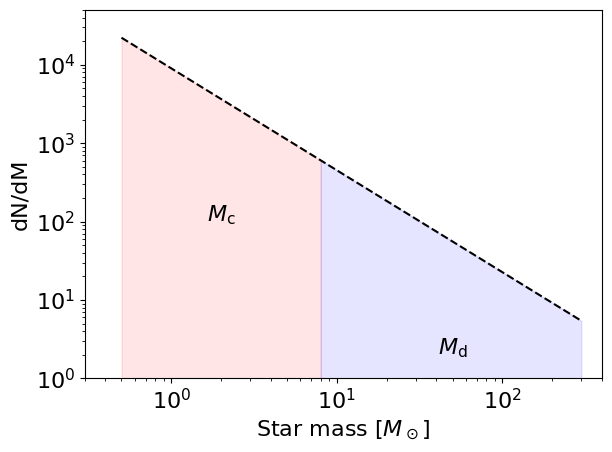
\includegraphics[scale=0.7]{sink_imf}
  \caption{This figure shows an IMF split into two parts: the continuous (orange) with mass and the discrete (blue) part with respective mass $M_c$ and $M_d$. The separating mass is called $m_t$. \emph{Source}: Roduit Darwin}
  \label{fig:sink_imf}
\end{figure}

Let us define $M_c$ the mass of the continuous part of the IMF and $M_d$ the mass of the discrete part by the following equation:
%
\begin{equation}
    M_c =  \int_{m_\text{min}}^{m_t} \Phi(m) \dd m \quad \text{and} \quad  M_d =  \int_{m_t}^{m_\text{max}} \Phi(m) \dd m \, ,
\end{equation}
%
where $\Phi(m)$ is the initial mass function. 

Similarly, we can define $N_c$ as the number of stars in the continuous part of the IMF and $N_d$ as the one in the discrete part:
%
\begin{equation}
    N_c =  \int_{m_\text{min}}^{m_t} \frac{\Phi(m)}{m} \dd m \quad \text{and} \quad  N_d =  \int_{m_t}^{m_\text{max}} \frac{\Phi(m)}{m} \dd m \, .
\end{equation}
%
Another important definition is the number of particles (not stars) $N_{\text{SP}}$ of mass $m_{\text{SP}}$ that will populate the continuous part of the IMF. Thus, the total number of stars that the IMF will generate is:
%
\begin{equation}
    N_{\text{tot}} = N_{\text{SP}} + N_d \, .
\end{equation}
%
$N_{\text{SP}}$ is obtained by dividing the mass $M_c$ of the continuous part of the IMF by the mass of the stellar particle $m_{\text{SP}}$:
%
\begin{equation}
    N_{\text{SP}} = \frac{M_c}{m_{\text{SP}}} \, .
\end{equation}
%
Now, we need to find the probability $P_c$ to spawn a star particle of mass $m_\text{SP}$ and $P_c$ the probability to spawn individual stars representing the discrete part of the IMF. With all the above definitions, it is easy to find those probabilities. Indeed, $P_c$ is given by:
%
\begin{equation}
    P_c = \frac{N_{\text{SP}}}{N_{\text{tot}}} = \frac{N_{\text{SP}}}{N_{\text{SP}} + N_d} \quad \text{and} \quad P_d = 1 - P_c \, .
\end{equation}
%
If we assume that only a star particle will contain all stars below $m_t$, i.e. $N_{\text{SP}} = 1$, we find:
%
\begin{equation}
    P_c = \frac{1}{1 + N_d} \, . 
\end{equation}
%
Therefore, the algorithm of the IMF sampling is presented in Algorithm \ref{algo:imf_sampling}. In this algorithm, we have assumed to have a function \texttt{sample\_IMF\_high()} that correctly samples the IMF for the discrete part. This algorithm is called whenever we need to set the target mass of the sink. So, it is called once a new sink is formed, if a sink exists in the inital conditions or after having spawned a star. \\

This algorithm is the same for populations II and III stars. However, the IMF parameters (mainly the minimal IMF mass and maximal IMF mass) and the two free parameters $m_t$ and $m_{SP}$ can vary.

\begin{algorithm}
  \begin{algorithmic}
      \State $\mathtt{random\_number} \gets \text{draw an random number in the interval }\left(0, 1 \right]$ 
      \If{$\mathtt{random\_number} < P_c$}
        \State $\mathtt{target\_mass} \gets m_{\text{SP}}$
      \Else
        \State $\mathtt{target\_mass} \gets \mathtt{sample\_IMF\_high()}$
      \EndIf
      \Return{$\mathtt{target\_mass}$}
\end{algorithmic}
\caption{IMF sampling algorithm, also called \texttt{sink\_update\_target\_mass()}. }\label{algo:imf_sampling}
\end{algorithm}


\end{document} %------------------------------------------------

%%% Local Variables:
%%% mode: latex
%%% TeX-master: t
%%% End:
